\documentclass[aspectratio=169]{beamer}
\usepackage[utf8]{inputenc}
\usepackage[T5]{fontenc}

\usetheme{Madrid}
\usecolortheme{default}
\setbeamertemplate{navigation symbols}{}

\usepackage{tikz}
\usetikzlibrary{shapes.geometric, arrows.meta, positioning, calc}
\usepackage{tabularx}
\usepackage{array}
\usepackage{graphicx}

\newcolumntype{Y}{>{\raggedright\arraybackslash}X}
\newcolumntype{L}[1]{>{\raggedright\arraybackslash}p{#1}}
\newcolumntype{C}[1]{>{\centering\arraybackslash}p{#1}}
\DeclareRobustCommand{\code}[1]{{\scriptsize\ttfamily #1}}
\renewcommand{\arraystretch}{1.14}

\title[Flow Table DPDK]{Hệ thống phân tải luồng và quản lý Flow Table hiệu năng cao}
\author{Trần Phúc Long}
\institute{VDT 2026}
\date{\today}

\begin{document}

\frame{\titlepage}

\begin{frame}{Bài toán và mục tiêu}
\small
\textbf{Vấn đề cần giải quyết}
\begin{itemize}
    \item Data plane không chỉ chuyển tiếp packet rời rạc; nó phải biết packet thuộc flow nào và giữ trạng thái của flow đó.
    \item Yêu cầu phân tải lưu lượng đều trên các CPU core để tối ưu hóa phần cứng
    \item Giới hạn của Linux kernel sinh ra nhiều overhead khi xử lí gói tin. 
\end{itemize}

\vspace{0.15cm}
\textbf{Mục tiêu xây dựng Flow Table}
\begin{itemize}
    \item Nhận IPv4 TCP/UDP, trích xuất 5-tuple, lookup hoặc tạo flow, rồi chuyển packet đến đúng worker.
    \item Giữ flow affinity: packet cùng flow đi về cùng worker.
    \item Có aging, overload replacement, SPI rule, hot reload rule và thống kê runtime.
    \item Flow Table khoảng 1 triệu entry benchmark bằng testpmd/memif.
\end{itemize}
\end{frame}

\begin{frame}{Kiến trúc tổng quan}
\centering
\resizebox{0.95\textwidth}{!}{%
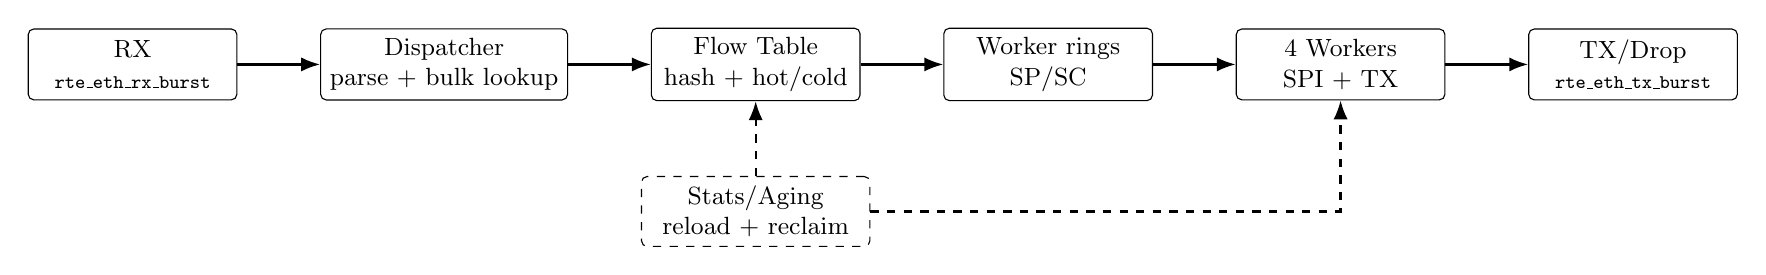
\begin{tikzpicture}[
    node distance=0.72cm and 1.05cm,
    box/.style={draw, rounded corners=2pt, minimum width=2.65cm, minimum height=0.9cm, align=center, font=\small},
    note/.style={draw, dashed, rounded corners=2pt, minimum width=2.9cm, minimum height=0.75cm, align=center, font=\small},
    arr/.style={-{Latex[length=2.4mm]}, thick}
]
\node[box] (rx) {RX\\\code{rte\_eth\_rx\_burst}};
\node[box, right=of rx] (disp) {Dispatcher\\parse + bulk lookup};
\node[box, right=of disp] (ft) {Flow Table\\hash + hot/cold};
\node[box, right=of ft] (rings) {Worker rings\\SP/SC};
\node[box, right=of rings] (workers) {4 Workers\\SPI + TX};
\node[box, right=of workers] (tx) {TX/Drop\\\code{rte\_eth\_tx\_burst}};
\node[note, below=0.95cm of ft] (stats) {Stats/Aging\\reload + reclaim};

\draw[arr] (rx) -- (disp);
\draw[arr] (disp) -- (ft);
\draw[arr] (ft) -- (rings);
\draw[arr] (rings) -- (workers);
\draw[arr] (workers) -- (tx);
\draw[arr, dashed] (stats.north) -- (ft.south);
\draw[arr, dashed] (stats.east) -| (workers.south);
\end{tikzpicture}%
}

\vspace{0.15cm}
\scriptsize
\begin{tabularx}{\textwidth}{|L{2.6cm}|Y|}
\hline
\textbf{Thành phần} & \textbf{Nhiệm vụ chính trong code hiện tại} \\
\hline
Dispatcher & Nhận burst, lọc non-IPv4/TCP/UDP, tạo 5-tuple, lookup/add flow, stamp metadata vào mbuf, enqueue sang ring worker. \\
\hline
Flow Table & Ánh xạ 5-tuple sang \code{flow\_idx}; state thật nằm trong hai mảng \code{hot[]} và \code{cold[]}. \\
\hline
Worker & Dequeue mbuf, kiểm tra \code{flow\_gen}, chạy SPI rule, cập nhật protocol counter, TX hoặc drop. \\
\hline
Stats/Aging & Reload rule, aging flow hết hạn, pressure maintenance, RCU reclaim và tổng hợp per-lcore stats. \\
\hline
\end{tabularx}
\end{frame}

\begin{frame}{Thiết kế lưu trữ Flow Table}
\small
\centering
\resizebox{0.86\textwidth}{!}{%
\begin{tikzpicture}[
    node distance=0.75cm and 1.1cm,
    box/.style={draw, rounded corners=2pt, minimum width=3.0cm, minimum height=0.85cm, align=center, font=\small},
    arr/.style={-{Latex[length=2.3mm]}, thick}
]
\node[box] (key) {5-tuple key\\src/dst IP, port, proto};
\node[box, right=of key] (hash) {\code{rte\_hash}\\CRC + LF flags};
\node[box, right=of hash] (idx) {\code{flow\_idx}\\slot id};
\node[box, above right=0.55cm and 1.0cm of idx] (hot) {\code{hot[flow\_idx]}\\dữ liệu hay chạm};
\node[box, below right=0.55cm and 1.0cm of idx] (cold) {\code{cold[flow\_idx]}\\mô tả flow};

\draw[arr] (key) -- (hash);
\draw[arr] (hash) -- (idx);
\draw[arr] (idx) -- (hot);
\draw[arr] (idx) -- (cold);
\end{tikzpicture}%
}

\vspace{0.2cm}
\begin{columns}[T]
\column{0.48\textwidth}
\textbf{Hot data}
\begin{itemize}
    \item \code{last\_seen}: dispatcher cập nhật trên hit/miss; aging đọc để timeout.
    \item \code{flow\_gen}: generation của slot, chống stale metadata.
    \item \code{worker\_id}: giữ flow affinity sau lần add đầu tiên.
\end{itemize}

\column{0.48\textwidth}
\textbf{Cold data}
\begin{itemize}
    \item \code{src\_ip}, \code{dst\_ip}, \code{src\_port}, \code{dst\_port}.
    \item \code{protocol}, \code{create\_time}.
    \item Worker dùng cho SPI và protocol accounting.
\end{itemize}
\end{columns}

\vspace{0.1cm}
\footnotesize
\textbf{Lý do tách hot/cold:} dispatcher hit path chỉ cần timestamp, worker và generation; IP/port/protocol không bị kéo vào cache trên mỗi hit.
\end{frame}

\begin{frame}{Flow Table: lookup và add bình thường}
\small
\centering
\resizebox{0.93\textwidth}{!}{%
\begin{tikzpicture}[
    node distance=0.72cm and 0.9cm,
    box/.style={draw, rounded corners=2pt, minimum width=2.9cm, minimum height=0.85cm, align=center, font=\small},
    decision/.style={draw, diamond, aspect=2.1, align=center, font=\small},
    arr/.style={-{Latex[length=2.2mm]}, thick}
]
\node[box] (parse) {Parse packet\\ra 5-tuple};
\node[box, right=of parse] (lookup) {Bulk lookup\\\code{rte\_hash}};
\node[decision, right=of lookup] (hit) {Hit?};
\node[box, above right=0.65cm and 0.7cm of hit] (hitpath) {Đọc \code{worker\_id}\\đọc \code{flow\_gen}};
\node[box, below right=0.65cm and 0.7cm of hit] (misspath) {Add key\\\code{rte\_hash\_add\_key}};
\node[box, right=1.55cm of hit] (publish) {Update/publish\\\code{hot/cold}};
\node[box, right=of publish] (stamp) {Stamp mbuf\\idx + gen};
\node[box, right=of stamp] (ring) {Enqueue\\worker ring};

\draw[arr] (parse) -- (lookup);
\draw[arr] (lookup) -- (hit);
\draw[arr] (hit) -- node[above, font=\small]{Có} (hitpath);
\draw[arr] (hit) -- node[below, font=\small]{Không} (misspath);
\draw[arr] (hitpath) -- (publish);
\draw[arr] (misspath) -- (publish);
\draw[arr] (publish) -- (stamp);
\draw[arr] (stamp) -- (ring);
\end{tikzpicture}%
}

\vspace{0.25cm}
\begin{itemize}
    \item \textbf{Hit path:} lấy \code{worker\_id}, đọc \code{flow\_gen}, cập nhật \code{last\_seen}, rồi chuyển mbuf sang worker.
    \item \textbf{Miss path bình thường:} add key, tăng \code{flow\_gen}, ghi cold data, chọn worker bằng hash của 5-tuple modulo 4, rồi store \code{last\_seen} cuối cùng.
    \item \textbf{Duplicate trong cùng burst:} dispatcher lưu kết quả đã resolve để packet trùng 5-tuple trong một burst dùng lại cùng flow vừa add.
\end{itemize}
\end{frame}

\begin{frame}{Aging flow và QSBR RCU}
\small
\begin{columns}[T]
\column{0.49\textwidth}
\textbf{Aging chạy trong stats thread}
\begin{itemize}
    \item Mỗi tick sleep \code{AGING\_INTERVAL\_US}; hiện là \(1/8\) giây.
    \item Mỗi tick scan khoảng \code{storage\_entries / 8} bằng \code{rte\_hash\_iterate}.
    \item Flow bị coi là hết hạn nếu không có packet mới quá \code{FLOW\_TIMEOUT\_SEC = 5} giây.
    \item Trước khi delete, code recheck \code{last\_seen}; nếu packet mới vừa đến thì không xóa.
\end{itemize}

\column{0.49\textwidth}
\textbf{QSBR RCU dùng để làm gì?}
\begin{itemize}
    \item Dispatcher và stats thread register QSBR.
    \item Delete hash entry được defer; reclaim chỉ chạy sau quiescent state.
    \item Stats thread offline trong lúc sleep để không giữ reader giả.
    \item RCU bảo vệ vòng đời entry trong hash, không tự bảo vệ ý nghĩa của \code{hot/cold} side arrays.
\end{itemize}
\end{columns}

\vspace{0.2cm}
\centering
\resizebox{0.78\textwidth}{!}{%
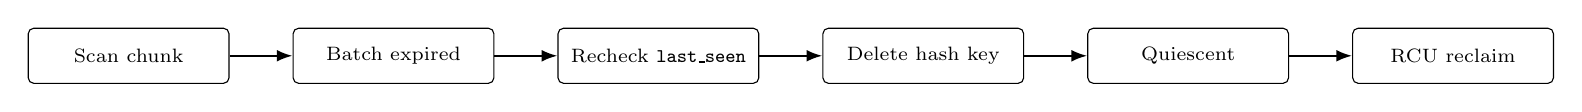
\begin{tikzpicture}[
    node distance=0.65cm and 0.8cm,
    box/.style={draw, rounded corners=2pt, minimum width=2.55cm, minimum height=0.7cm, align=center, font=\scriptsize},
    arr/.style={-{Latex[length=2mm]}, thick}
]
\node[box] (scan) {Scan chunk};
\node[box, right=of scan] (batch) {Batch expired};
\node[box, right=of batch] (recheck) {Recheck \code{last\_seen}};
\node[box, right=of recheck] (delete) {Delete hash key};
\node[box, right=of delete] (qs) {Quiescent};
\node[box, right=of qs] (reclaim) {RCU reclaim};
\draw[arr] (scan) -- (batch);
\draw[arr] (batch) -- (recheck);
\draw[arr] (recheck) -- (delete);
\draw[arr] (delete) -- (qs);
\draw[arr] (qs) -- (reclaim);
\end{tikzpicture}%
}
\end{frame}

\begin{frame}{Replacement policy khi overload flow}
\small
\begin{columns}[T]
\column{0.48\textwidth}
\textbf{Pressure maintenance}
\begin{itemize}
    \item Watermark: \code{PRESSURE} 92\%, \code{AGGRESSIVE} 96\%, \code{CRITICAL} 99\%.
    \item Stats thread scan bằng \code{pressure\_iter}, tách khỏi \code{aging\_iter}.
    \item Candidate phải hợp lệ: position đúng, \code{last\_seen != 0}, generation khớp, idle đủ theo mode.
    \item Nếu chưa cần evict ngay, candidate được đẩy vào victim cache.
\end{itemize}

\column{0.48\textwidth}
\textbf{Dispatcher khi add flow fail}
\begin{itemize}
    \item Pop tối đa \code{FLOW\_REPLACEMENT\_RETRIES = 8} victim từ cache.
    \item Validate lại key, position, generation và idle trước khi delete.
    \item Quiescent + reclaim một phần, rồi retry add flow mới.
    \item Nếu cache không dùng được, emergency sampling chọn vài slot ngẫu nhiên.
\end{itemize}
\end{columns}

\vspace{0.15cm}
\scriptsize
\begin{tabularx}{\textwidth}{|L{2.5cm}|L{2.1cm}|Y|}
\hline
\textbf{Cơ chế} & \textbf{Giá trị} & \textbf{Ý nghĩa} \\
\hline
Victim cache & 8192 entry & Ring SP/SC chứa victim đã được stats thread chuẩn bị. \\
\hline
Packing & 64 bit & Pack \code{position} + \code{flow\_gen}; key được dựng lại từ \code{cold[position]}. \\
\hline
Tradeoff & Không exact LRU & Đổi độ chính xác eviction lấy hot path nhẹ hơn; candidate stale phải validate lại. \\
\hline
\end{tabularx}
\end{frame}

\begin{frame}{Vòng đời packet: zero-copy và \code{flow\_gen}}
\small
\centering
\resizebox{0.9\textwidth}{!}{%
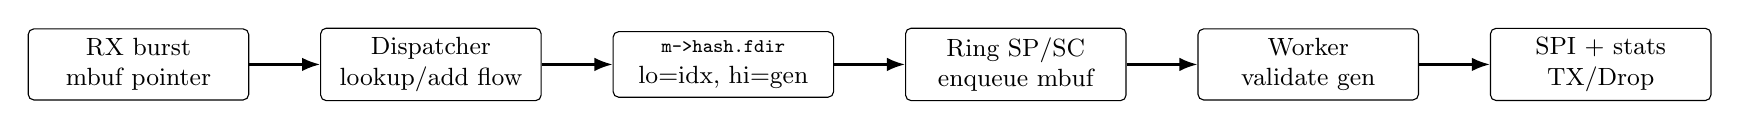
\begin{tikzpicture}[
    node distance=0.75cm and 0.9cm,
    box/.style={draw, rounded corners=2pt, minimum width=2.8cm, minimum height=0.8cm, align=center, font=\small},
    arr/.style={-{Latex[length=2.3mm]}, thick}
]
\node[box] (rx) {RX burst\\mbuf pointer};
\node[box, right=of rx] (dispatch) {Dispatcher\\lookup/add flow};
\node[box, right=of dispatch] (stamp) {\code{m->hash.fdir}\\lo=idx, hi=gen};
\node[box, right=of stamp] (ring) {Ring SP/SC\\enqueue mbuf};
\node[box, right=of ring] (worker) {Worker\\validate gen};
\node[box, right=of worker] (spi) {SPI + stats\\TX/Drop};

\draw[arr] (rx) -- (dispatch);
\draw[arr] (dispatch) -- (stamp);
\draw[arr] (stamp) -- (ring);
\draw[arr] (ring) -- (worker);
\draw[arr] (worker) -- (spi);
\end{tikzpicture}%
}

\vspace{0.25cm}
\begin{itemize}
    \item Dispatcher không copy payload; nó truyền chính con trỏ \code{struct rte\_mbuf *} sang worker qua \code{rte\_ring\_enqueue\_burst}.
    \item Worker không lookup hash lại; nó đọc \code{flow\_idx} và \code{flow\_gen} trong mbuf để lấy cold-data snapshot.
    \item \code{flow\_gen} cần thiết vì slot có thể bị aging/replacement rồi được flow mới dùng lại trong lúc packet cũ vẫn đang nằm ở worker ring.
    \item Nếu generation lệch, worker parse lại packet để lấy cold-data tạm thời thay vì đọc nhầm metadata của flow mới.
\end{itemize}
\end{frame}

\begin{frame}{Thống kê runtime}
\small
\begin{itemize}
    \item Mỗi lcore có một vùng \code{struct lcore\_stats} cache-aligned; dispatcher, worker và stats thread tự cập nhật counter của mình.
    \item Stats thread gọi \code{stats\_collect\_totals()} để cộng các lcore theo chu kỳ, không bắt hot path dùng atomic counter toàn cục.
    \item Các metric chính: RX/TX PPS, Mbps, active flows, created/deleted flows, timeout delete, pressure evict, ring drop, TX drop, hash add fail.
    \item SPI metrics: forwarded, dropped, rule checks, rule version và protocol counters HTTP/HTTPS/DNS/TCP/UDP/OTHER.
    \item Tradeoff: telemetry là snapshot gần đúng theo chu kỳ, không phải trạng thái transactional tuyệt đối tại một nanosecond.
\end{itemize}
\end{frame}

\begin{frame}{Kết quả chức năng}
\scriptsize
\begin{tabularx}{\textwidth}{|L{2.8cm}|Y|Y|}
\hline
\textbf{Ca kiểm thử} & \textbf{Cách mô phỏng} & \textbf{Điều xác nhận} \\
\hline
Same flow reuse & PCAP 10 packet cùng 5-tuple & Chỉ tạo 1 flow, packet được forward. \\
\hline
Unique flow creation & PCAP 32 packet khác 5-tuple & Tạo đúng 32 flow. \\
\hline
Rule drop SSH & PCAP có TCP/22 và port khác & Rule DROP làm rơi đúng packet SSH. \\
\hline
Protocol accounting & PCAP HTTP, HTTPS, DNS, TCP khác, UDP khác & Counter protocol khớp kỳ vọng. \\
\hline
Aging cleanup & Một flow, chạy quá timeout & Flow được tạo rồi bị xóa bởi aging. \\
\hline
Non-TCP/UDP filtered & PCAP ICMP và ARP & Không tạo flow, tăng filtered counter. \\
\hline
Hot reload & TCP/8443 lặp, đổi rule rồi gửi \code{SIGUSR1} & Rule version tăng, có forward trước reload và drop sau reload. \\
\hline
Overload replacement & Hash nhỏ \code{HASH\_ENTRIES=64}, thêm flow đến khi đầy & Evict victim và add flow mới sau reclaim. \\
\hline
\end{tabularx}

\vspace{0.15cm}
\footnotesize
Các test xác nhận logic và regression trong môi trường software-only; chúng chưa thay thế benchmark bằng NIC thật.
\end{frame}

\begin{frame}{Kết quả hiệu năng: flow sweep}
\small
\textbf{Kịch bản:} \code{dpdk-testpmd} chế độ \code{flowgen}, kết nối với FlowCore qua \code{memif}. Throughput dùng TX PPS vì đây là số packet đã đi hết pipeline.

\vspace{0.2cm}
\centering
\scriptsize
\begin{tabularx}{0.98\textwidth}{|C{1.75cm}|C{2.05cm}|C{1.95cm}|C{1.75cm}|>{\centering\arraybackslash}X|}
\hline
\textbf{Flow cấu hình} & \textbf{TX throughput} & \textbf{Active flow} & \textbf{Create/s} & \textbf{Delete/s} \\
\hline
500k & 9.22 Mpps & 500k & 0 & 0 \\
\hline
1.0M & 9.07 Mpps & 1.00M & 0 & 0 \\
\hline
1.1M & 3.32 Mpps & 1.03M & 407k & 369k \\
\hline
1.2M & 2.35 Mpps & 1.03M & 481k & 379k \\
\hline
1.5M & 1.28 Mpps & 1.01M & 495k & 407k \\
\hline
2.0M & 0.78 Mpps & 1.03M & 444k & 359k \\
\hline
\end{tabularx}
\end{frame}

\begin{frame}{Đọc kết quả hiệu năng}
\small
\begin{itemize}
    \item 500k và 1M flow: throughput khoảng 9 Mpps, TX drop = 0, ring drop = 0, hash add fail = 0.
    \item Từ 1.1M flow trở lên: workload vượt dung lượng hiệu dụng của Flow Table, pressure chuyển sang \code{AGGRESSIVE}.
    \item Active flow thực tế được giữ quanh 1.01--1.03M flow; snapshot cao nhất là 1,032,655 active flow ở kịch bản 1.2M.
    \item Throughput giảm trong vùng overload vì hệ thống phải add flow mới, evict victim, retry add và reclaim liên tục.
    \item Trong các snapshot này, TX drop và ring drop đều bằng 0; replacement fail cũng bằng 0.
\end{itemize}

\vspace{0.1cm}
\centering
\scriptsize
\begin{tabularx}{0.95\textwidth}{|C{1.5cm}|C{2.0cm}|C{2.0cm}|C{2.1cm}|C{1.6cm}|}
\hline
\textbf{Flow} & \textbf{Pressure} & \textbf{Hash fail/s} & \textbf{Replacement attempts} & \textbf{TX/Ring drop} \\
\hline
500k & NORMAL & 0 & 0 & 0/0 \\
\hline
1.0M & PRESSURE & 0 & 0 & 0/0 \\
\hline
1.1M & AGGRESSIVE & 2,092 & 80,450 & 0/0 \\
\hline
1.2M & AGGRESSIVE & 4,633 & 76,109 & 0/0 \\
\hline
1.5M & AGGRESSIVE & 7,868 & 134,327 & 0/0 \\
\hline
2.0M & AGGRESSIVE & 6,075 & 51,794 & 0/0 \\
\hline
\end{tabularx}
\end{frame}

\begin{frame}{Nhược điểm còn tồn tại}
\small
\begin{itemize}
    \item Số worker đang cố định ở compile-time: \code{NUM\_WORKERS = 4}.
    \item Parser hiện tập trung vào IPv4 TCP/UDP; chưa hỗ trợ đầy đủ IPv6, VLAN, fragmented IPv4, scattered mbuf và jumbo frame.
    \item SPI rule matching tuyến tính theo số rule; rule set lớn sẽ cần indexing hoặc DPDK ACL.
    \item Aging dùng hash iterator theo chunk; khi scale lên nhiều triệu flow hơn nữa, timing wheel hoặc expiry bucket sẽ ổn định hơn.
    \item Replacement không phải exact LRU; nó là policy thực dụng dựa trên idle time, iterator và victim cache.
    \item Benchmark hiện dùng testpmd/memif trên cùng máy; chưa có kết quả với NIC thật, RSS, NUMA pinning và latency tail.
\end{itemize}
\end{frame}

\begin{frame}{Hướng phát triển}
\small
\begin{itemize}
    \item Cho phép cấu hình runtime số worker, kích thước Flow Table và tham số pressure/aging.
    \item Thêm RSS/multi-dispatcher để mở rộng theo nhiều RX queue và nhiều NUMA node.
    \item Nâng cấp aging bằng timing wheel hoặc expiry bucket để giảm phụ thuộc vào hash iterator.
    \item Tối ưu SPI bằng phân nhóm rule theo protocol/port hoặc dùng DPDK ACL.
    \item Xuất thống kê dạng JSON để phục vụ dashboard và kiểm thử tự động.
    \item Bổ sung hỗ trợ IPv6, VLAN, fragmented packet và scattered mbuf.
    \item Đo lại trên NIC thật với traffic generator để có số liệu line-rate và latency tail.
\end{itemize}
\end{frame}

\begin{frame}
\centering
\Huge \textbf{Cảm ơn anh/chị đã lắng nghe}\\
\vspace{0.8cm}
\Large Q\&A
\end{frame}

\end{document}
